\section{Código de ejemplo de una aplicación}

\begin{frame}{Ejemplo}
	\begin{block}{Enviar mensajes}
		Esta aplicación sirve para enviar texto desde una pestaña de Google Chrome y mostrarlo en una pantalla conectada a un Chromecast.
	\end{block}
	
	\begin{block}{ }
		Esta aplicación consta de dos partes: la del emisor (Google Chrome) y la del receptor (Chromecast).
		Ambas son web apps en HTML que cargan un código JavaScript.
		Para ejecutarla debemos alojarla en un servidor.
	\end{block}
\end{frame}



\begin{frame}{Creando servidor en el puerto 8000}
	\begin{figure}[H]
		\centering
		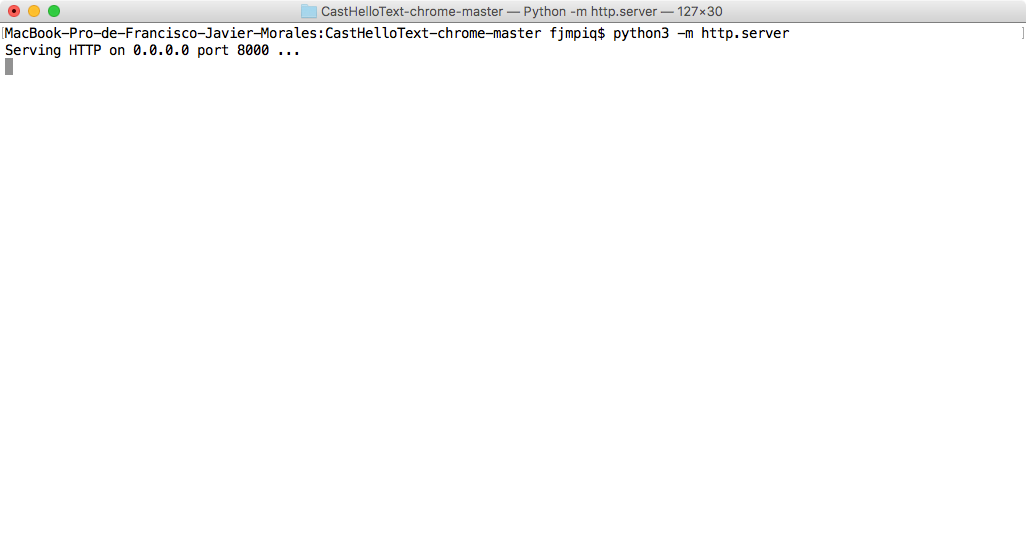
\includegraphics[width=1.05\textwidth]{./Imagenes/creando_servidor.png}
	\end{figure}
\end{frame}



\begin{frame}{Aplicación emisora}
	\begin{block}{Chromehellotext.html}
		Desde Chrome, accedemos a la aplicación emisora (chromehellotext.html).
	\end{block}
\end{frame}



\begin{frame}{Directorio del servidor}
	\begin{figure}[H]
		\centering
		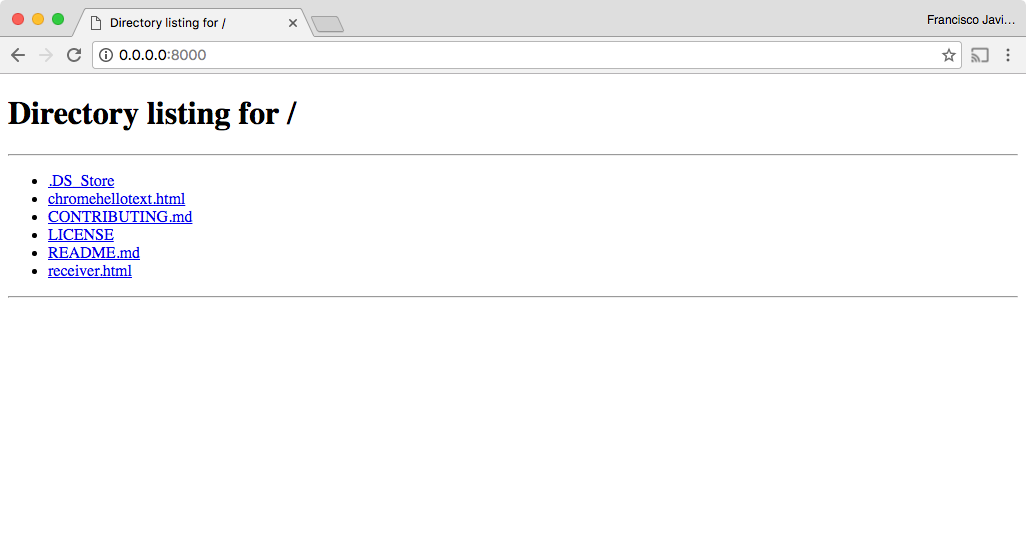
\includegraphics[width=1.05\textwidth]{./Imagenes/directorylisting.png}
	\end{figure}
\end{frame}



\begin{frame}{Aplicación emisora}
	\begin{figure}[H]
		\centering
		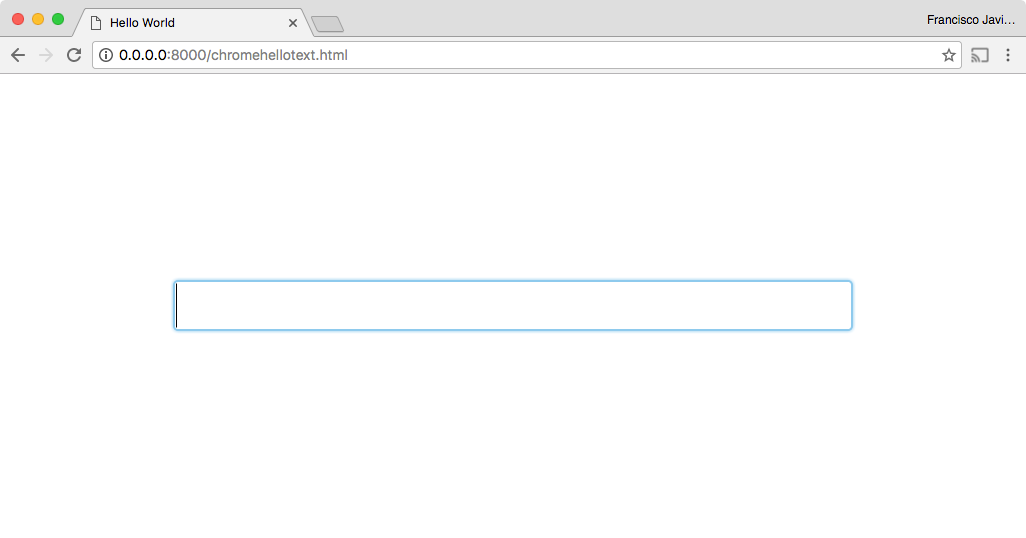
\includegraphics[width=1.05\textwidth]{./Imagenes/emisor1.png}
	\end{figure}
\end{frame}



\begin{frame}{Enviando contenido}
	\begin{block}{ }
		A continuación, desde la extensión de Google Cast, seleccionamos enviar el contenido de la aplicación a nuestro Chromecast.
	\end{block}
\end{frame}



\begin{frame}{Selección del Chromecast}
	\begin{block}{mDNS}
		Ahora es donde actúa mDNS
	\end{block}
	\vspace{0.5cm}
	\begin{figure}[H]
		\centering
		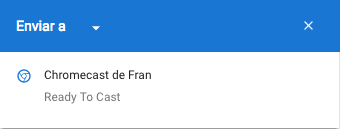
\includegraphics[width=0.75\textwidth]{./Imagenes/seleccion.png}
	\end{figure}
\end{frame}



\begin{frame}{Receiver.html}
	\begin{block}{ }
		En ese momento, debería cargar en el Chromecast la aplicación receptora (receiver.html).
		Ya podemos escribir texto en el emisor y, al pulsar intro, debería aparecer en el televisor.
	\end{block}
\end{frame}


